\documentclass[conference]{IEEEtran}
\IEEEoverridecommandlockouts
% Supplied IEEE conference template; anonymous author block retained.
% Build from the project root using scripts/build_paper.py.
% Empirical numbers and tables are generated from final artifacts.
\usepackage[T1]{fontenc}
\usepackage{cite}
\usepackage{amsmath,amssymb,amsfonts}
\usepackage{graphicx}
\usepackage{textcomp}
\usepackage{xcolor}
\usepackage{booktabs}
\usepackage[hyphens]{url}
\def\BibTeX{{\rm B\kern-.05em{\sc i\kern-.025em b}\kern-.08em
    T\kern-.1667em\lower.7ex\hbox{E}\kern-.125emX}}
% Generated from final canonical artifacts; do not hand-edit.
\newcommand{\BaseIID}{0.9815}
\newcommand{\BaseIIDPct}{98.15}
\newcommand{\BaseRec}{0.9871}
\newcommand{\BaseRecPct}{98.71}
\newcommand{\BaseHB}{0.4158}
\newcommand{\BaseHBPct}{41.58}
\newcommand{\BaseExt}{0.2067}
\newcommand{\BaseExtPct}{20.67}
\newcommand{\BaseObf}{0.9857}
\newcommand{\BaseObfPct}{98.57}
\newcommand{\BaseDom}{0.9033}
\newcommand{\BaseDomPct}{90.33}
\newcommand{\BaseStruct}{0.7748}
\newcommand{\BaseStructPct}{77.48}
\newcommand{\CurIID}{0.9828}
\newcommand{\CurIIDPct}{98.28}
\newcommand{\CurRec}{0.9892}
\newcommand{\CurRecPct}{98.92}
\newcommand{\CurHB}{0.0587}
\newcommand{\CurHBPct}{5.87}
\newcommand{\CurExt}{0.1846}
\newcommand{\CurExtPct}{18.46}
\newcommand{\CurObf}{0.9921}
\newcommand{\CurObfPct}{99.21}
\newcommand{\CurDom}{0.9131}
\newcommand{\CurDomPct}{91.31}
\newcommand{\CurStruct}{0.5359}
\newcommand{\CurStructPct}{53.59}
\newcommand{\RandIID}{0.9840}
\newcommand{\RandIIDPct}{98.40}
\newcommand{\RandRec}{0.9877}
\newcommand{\RandRecPct}{98.77}
\newcommand{\RandHB}{0.2015}
\newcommand{\RandHBPct}{20.15}
\newcommand{\RandExt}{0.0731}
\newcommand{\RandExtPct}{7.31}
\newcommand{\RandObf}{0.9891}
\newcommand{\RandObfPct}{98.91}
\newcommand{\RandDom}{0.8899}
\newcommand{\RandDomPct}{88.99}
\newcommand{\RandStruct}{0.4356}
\newcommand{\RandStructPct}{43.56}
\newcommand{\PGIID}{0.9826}
\newcommand{\PGIIDPct}{98.26}
\newcommand{\PGRec}{0.9869}
\newcommand{\PGRecPct}{98.69}
\newcommand{\PGHB}{0.1384}
\newcommand{\PGHBPct}{13.84}
\newcommand{\PGExt}{0.0423}
\newcommand{\PGExtPct}{4.23}
\newcommand{\PGObf}{0.9877}
\newcommand{\PGObfPct}{98.77}
\newcommand{\PGDom}{0.8839}
\newcommand{\PGDomPct}{88.39}
\newcommand{\PGStruct}{0.3754}
\newcommand{\PGStructPct}{37.54}
\newcommand{\CurCuratedFPR}{0.0150}
\newcommand{\PGCuratedFPR}{0.1717}
\newcommand{\BaseHBDropPP}{27.75}
\newcommand{\BaseHBDropRel}{66.7}
\newcommand{\BaseExtDropPP}{16.44}
\newcommand{\BaseExtDropRel}{79.5}
\newcommand{\BaseIIDChangePP}{+0.12}
\newcommand{\BaseRecChangePP}{-0.03}
\newcommand{\BaseDomChangePP}{-1.94}
\newcommand{\BaseStructChangePP}{-39.94}
\newcommand{\RandHBDropPP}{6.31}
\newcommand{\RandHBDropRel}{31.3}
\newcommand{\RandExtDropPP}{3.08}
\newcommand{\RandExtDropRel}{42.1}
\newcommand{\RandIIDChangePP}{-0.13}
\newcommand{\RandRecChangePP}{-0.09}
\newcommand{\RandDomChangePP}{-0.60}
\newcommand{\RandStructChangePP}{-6.03}
\newcommand{\CurHBDropPP}{-7.97}
\newcommand{\CurHBDropRel}{-135.9}
\newcommand{\CurExtDropPP}{14.23}
\newcommand{\CurExtDropRel}{77.1}
\newcommand{\CurIIDChangePP}{-0.01}
\newcommand{\CurRecChangePP}{-0.23}
\newcommand{\CurDomChangePP}{-2.92}
\newcommand{\CurStructChangePP}{-16.06}
\newcommand{\BaseHBCI}{[0.2007,\,0.3512]}
\newcommand{\BaseExtCI}{[0.1173,\,0.2144]}
\newcommand{\RandHBCI}{[-0.0050,\,0.1408]}
\newcommand{\RandExtCI}{[0.0096,\,0.0548]}
\newcommand{\CurHBCI}{[-0.1267,\,-0.0379]}
\newcommand{\CurExtCI}{[0.0933,\,0.1933]}
\newcommand{\PreserveIIDCI}{[-0.0006,\,0.0033]}
\newcommand{\PreserveRecCI}{[-0.0036,\,0.0043]}
\newcommand{\PreserveObfCI}{[-0.0059,\,0.0148]}
\newcommand{\NTrain}{27093}
\newcommand{\NVal}{3989}
\newcommand{\NIID}{3918}
\newcommand{\NHB}{808}
\newcommand{\NReleasedHB}{1472}
\newcommand{\NWithheld}{664}
\newcommand{\NObf}{405}
\newcommand{\NDomain}{2000}
\newcommand{\NStruct}{1998}
\newcommand{\NCandidatesBefore}{17535}
\newcommand{\NCandidates}{17400}
\newcommand{\NExactRemoved}{117}
\newcommand{\NNearRemoved}{18}
\newcommand{\NCurAug}{343}
\newcommand{\NReviewed}{2927}
\newcommand{\NApproved}{2923}
\newcommand{\NRejected}{3}
\newcommand{\NAmbiguous}{1}
\newcommand{\NDollySelected}{429}
\newcommand{\NOasstSelected}{571}
\newcommand{\NOverlap}{213}
\newcommand{\NLastRank}{1004}
\newcommand{\NExternal}{208}
\newcommand{\NCuratedHB}{600}
\newcommand{\PrimaryK}{1000}
\newcommand{\NSeeds}{5}
\newcommand{\NSelectors}{3}
\newcommand{\MinChars}{20}
\newcommand{\NEpochs}{2}
\newcommand{\NBatch}{16}
\newcommand{\MaxLength}{256}
\newcommand{\NRuns}{30}
\newcommand{\Threshold}{0.5}
\newcommand{\LeakThreshold}{0.90}
\newcommand{\WeightDecay}{0.01}
\newcommand{\MaxGradNorm}{1.0}
\newcommand{\BootstrapN}{10000}
\newcommand{\HardPGMean}{0.198910}
\newcommand{\HardPGMedian}{0.016738}
\newcommand{\HardPGQThree}{0.330759}
\newcommand{\HardPGFlagN}{172}
\newcommand{\HardRandMean}{0.058424}
\newcommand{\HardRandMedian}{0.000903}
\newcommand{\HardRandQThree}{0.003713}
\newcommand{\HardRandFlagN}{53}
\newcommand{\HardCurMean}{0.493198}
\newcommand{\HardCurMedian}{0.651523}
\newcommand{\HardCurQThree}{0.670925}
\newcommand{\HardCurFlagN}{195}
\newcommand{\KSmallHBPct}{12.40}
\newcommand{\KSmallExtPct}{5.38}
\newcommand{\KMediumHBPct}{16.88}
\newcommand{\KMediumExtPct}{3.46}
\newcommand{\SourceDollyDollyFPR}{0.0000}
\newcommand{\SourceDollyOasstFPR}{0.2095}
\newcommand{\SourceOasstDollyFPR}{0.0196}
\newcommand{\SourceOasstOasstFPR}{0.0619}
\newcommand{\SourceSeedN}{3}
\newcommand{\NDollyExternal}{68}
\newcommand{\NOasstExternal}{140}
\newcommand{\FixedFP}{245.0}
\newcommand{\NewFP}{20.8}

\title{ProvGuard: Confusion-Selected Hard Negatives for Reducing Prompt-Injection Over-Defense under Distribution Shift}
\author{\IEEEauthorblockN{Anonymous Authors}}
\begin{document}
\maketitle

\begin{abstract}
Prompt-injection detectors can reject benign requests that resemble attacks despite high in-distribution accuracy. Hard-negative augmentation may reduce this over-defense on curated stress examples yet transfer poorly to externally sourced prompts. We study whether the provenance and selection of benign augmentation data explain this gap. ProvGuard ranks naturally occurring Dolly and OpenAssistant prompts by the mean injection probability of three baseline detectors, applies lexical leakage controls and two-pass automated semantic adjudication, and retrains the same DistilBERT classifier on the selected benign examples. We complete a five-seed comparison with an unaugmented baseline, curated hard negatives, and an equal-sized source/length-matched Random-Real control, plus nested size ablations. At a fixed threshold, external hard-benign false-positive rate falls from \BaseExtPct\% to \PGExtPct\%, a \BaseExtDropRel\% relative reduction. IID F1 changes from \BaseIIDPct\% to \PGIIDPct\%, while attack recall changes from \BaseRecPct\% to \PGRecPct\%. ProvGuard improves on Random-Real's \RandExtPct\% external false-positive rate, with a positive paired-bootstrap interval for the reduction; the aggregate mixed-set comparison remains inconclusive. Curated augmentation performs best on the curated-heavy aggregate, and domain-OOD F1 decreases under ProvGuard. These results support provenance-sensitive, target-distribution gains rather than universal superiority or a new detector architecture.
\end{abstract}
\begin{IEEEkeywords}
prompt injection, over-defense, hard-negative mining, false positives, provenance, data-centric robustness
\end{IEEEkeywords}

\section{Introduction}
Prompt injection attempts to redirect a language-model application through instructions that violate its intended task or trust boundary. Indirect injection places such instructions in external content consumed by the application~\cite{greshake}. A detector can screen that content before execution, but a useful screen must also accept benign discussion of attacks, system prompts, and security controls. Rejecting a request merely because it contains attack-associated wording imposes a usability cost.

High in-distribution (IID) performance can conceal this cost. Our unaugmented detector attains \BaseIIDPct\% IID F1 yet flags \BaseExtPct\% of the available externally sourced hard-benign prompts. Prior work documents over-defense from trigger-word bias~\cite{piguard} and sensitivity to benign-data provenance~\cite{pids}. Curated hard negatives can teach a detector to accept curated stress templates without adequately covering naturally occurring requests. This motivates a data-selection question rather than a new architecture:
\emph{Can naturally occurring benign prompts that a prompt-injection detector finds attack-like reduce over-defense on externally sourced benign inputs more effectively than generic benign augmentation, without materially weakening attack detection?}

ProvGuard selects relatively detector-confusing verified-benign prompts from Dolly and OpenAssistant. All arms retain the same classifier, original validation split, optimization settings, and threshold. An equal-sized, source/length-matched Random-Real control measures what targeted selection adds beyond realistic benign data. A curated arm reveals whether gains depend on evaluation provenance.

The evidence is mixed in an informative way. Random-Real already reduces external false positives substantially; targeted selection yields a further \RandExtDropPP{}-percentage-point reduction. Curated-HN instead achieves the lowest aggregate hard-benign rate on a population dominated by curated prompts. ProvGuard's advantage over Random-Real is supported on the targeted external subset, while the aggregate interval crosses zero. Our contributions are:
\begin{enumerate}
\item \textbf{A data-selection method:} ensemble-confusion ranking of naturally occurring prompts, with persisted lexical exclusion and recorded semantic validity decisions.
\item \textbf{A controlled study:} \NRuns{} DistilBERT runs across \NSeeds{} seeds, comparing baseline, curated, matched random, and three nested ProvGuard sizes.
\item \textbf{A target-distribution result:} external hard-benign FPR decreases from \BaseExtPct\% to \PGExtPct\%, and from Random-Real's \RandExtPct\%, while IID attack recall remains effectively unchanged.
\item \textbf{A qualified analysis:} paired uncertainty estimates, hardness distributions, error transitions, size sensitivity, and contrasting structural- and domain-OOD outcomes.
\end{enumerate}

\section{Related Work}
\subsection{Injection Detection and Over-Defense}
Greshake \emph{et al.} demonstrate how indirect injection crosses application trust boundaries~\cite{greshake}. DataSentinel formulates detection against adaptive injected prompts as minimax learning~\cite{datasentinel}. Such attacker-facing work addresses a different objective from accepting legitimate attack-adjacent requests; our study does not evaluate adaptive adversaries or end-to-end application security.

PIGuard introduces NotInject and a training strategy to reduce over-defense caused by trigger-word bias~\cite{piguard}. CAPTURE jointly examines attacks and benign cases in context-aware settings~\cite{capture}. PIDS-Bench measures hard-benign, obfuscated, domain-, and structural-shift behavior and reports provenance-sensitive effects of curated augmentation~\cite{pids}. We address its externally matched augmentation question with a matched real-data control. We do not compare directly with published full-coverage detector scores: the available public-text evaluation has different coverage, and no state-of-the-art claim follows.

\subsection{Hard Negatives and Data-Centric Robustness}
Hard-example mining is established, including online mining in object detection~\cite{ohem}. Shortcut learning provides a general explanation for high IID accuracy coupled with distribution-dependent failures~\cite{shortcuts}. ProvGuard's contribution is the controlled application of confusion-selected \emph{naturally occurring benign instruction data} to a specific provenance-sensitive failure, rather than invention of mining or proof of shortcut removal.

Dolly contains human-written instruction records~\cite{dolly}; OpenAssistant provides crowdsourced conversations~\cite{oasst,oasstcard}. Human origin does not establish a benign injection label. We therefore separate corpus extraction from semantic adjudication. DistilBERT~\cite{distilbert} remains the fixed primary architecture.

\section{Method}
\subsection{Scoring and Training Objective}
For input $x$, the classifier estimates $f_{\theta}(x)=P(y=1\mid x)$, where $y=1$ denotes injection and $y=0$ benign. Every evaluation uses $\hat y=\mathbb{I}[f_{\theta}(x)\geq\Threshold]$. Selector models are the unaugmented baselines with seeds $S=\{13,42,123\}$. Define
\begin{equation}
\begin{aligned}
h(x)&=\frac{1}{|S|}\sum_{s\in S}f_{\theta_s}(x),\\
H_K&=\operatorname{TopK}_{x\in B_{\mathrm{verified}}}h(x).
\end{aligned}
\label{eq:selection}
\end{equation}
Ranking is descending, with candidate identifier breaking ties. Each $H_K$ example receives benign label $0$, and the same classifier is fine-tuned on
\begin{equation}
D_{\mathrm{ProvGuard}}=D_{\mathrm{PIDS\ train}}\cup H_K.
\end{equation}
The predefined primary setting is $K=\PrimaryK$; nested $K=250$ and $500$ sets are ablations. A top-ranked example need not exceed the classifier threshold.

\begin{figure*}[t]
\centering
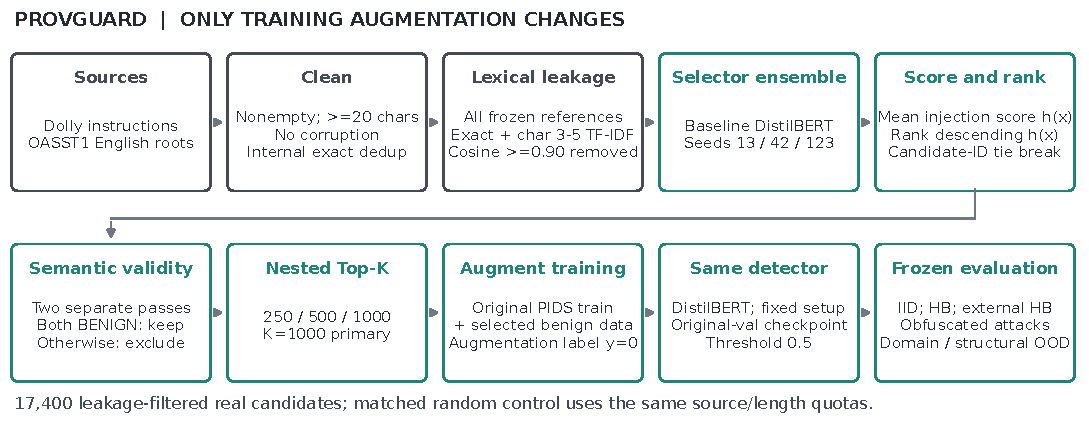
\includegraphics[width=\textwidth]{figures/paper/methodology.pdf}
\caption{ProvGuard changes training augmentation only. One persisted TF--IDF representation excludes lexical benchmark overlap; three baseline selectors rank candidate confusion; two separate automated adjudication passes establish operational benign eligibility. The fixed classifier and evaluation files are retained.}
\label{fig:method}
\end{figure*}

\subsection{Candidate Preparation and Lexical Exclusion}
Figure~\ref{fig:method} summarizes the pipeline. We use Dolly's instruction field without concatenating responses or context. OASST1 candidates are nondeleted, English, root-level prompter messages from its training split. We exclude empty texts, fragments shorter than \MinChars{} characters, and explicit corruption markers; normalized exact duplicates are removed internally. Retained text keeps its original formatting.

All accessible text from the frozen training, validation, and evaluation files forms the exclusion reference. Exact comparison lowercases and collapses whitespace. A character-boundary TF--IDF representation with $3$--$5$-grams is fitted \emph{once} on the canonical union of reference and potential augmentation texts, then persisted. Candidates with cosine similarity $\geq\LeakThreshold$ to a reference are removed. Construction and independent checks transform text with this same representation. Reference evaluation text is used solely for overlap exclusion, not as augmentation or a labeled selection signal; this unsupervised lexical representation does see the available benchmark text.

The \NCandidatesBefore{} cleaned real candidates lose \NExactRemoved{} exact and \NNearRemoved{} near overlaps, leaving \NCandidates{}. The valid curated augmentation has \NCurAug{} rows after the same policy. These controls prevent exact and high-similarity lexical overlap with available benchmark text but cannot guarantee complete semantic independence. Original benchmark files remain frozen.

\subsection{Automated Semantic Validity}
Two separately instantiated Codex reviewers read full candidate texts with numerical scores withheld. They label operational intent as BENIGN, INJECTION, or AMBIGUOUS. Benign security explanations, quotations, fiction, and imperatives remain eligible unless they direct the current model to override higher-priority instructions, reveal hidden prompts, bypass controls, or exfiltrate secrets. This is semantic adjudication, not a keyword ban or content-safety assessment.

Both passes must mark BENIGN for acceptance; either INJECTION rejects, and all other disagreement or uncertainty excludes. The passes review the top-ranked batch and additional independent random-control candidates: \NReviewed{} paired records yield \NApproved{} BENIGN, \NRejected{} INJECTION, and \NAmbiguous{} AMBIGUOUS decisions. The primary set reaches rank \NLastRank{} to retain \PrimaryK{} examples. Scores are hidden but ranked batch order is visible. Separate histories do not eliminate correlated model error, the exact serving model version was not exposed, and agreement is not human validation. Full texts, decisions, reasons, and procedure prompts are recorded for audit.

\subsection{Controls and Matching}
Baseline uses no added data. Curated-HN uses \NCurAug{} valid upstream constructed negatives. Random-Real draws \PrimaryK{} verified-benign real prompts independently of hardness: a fixed seed-42 permutation within corpus and full-candidate character-length quartiles supplies the first eligible records for each treatment quota. Both real arms contain \NDollySelected{} Dolly and \NOasstSelected{} OASST1 prompts. Their \NOverlap{}-example overlap is allowed, avoiding forced disjointness or easy-negative selection. Source/length matching does not establish syntactic equivalence. Curated-HN is a provenance control, not a size-matched mining control.

\section{Experimental Setup}
\subsection{Frozen Evaluation and Public Coverage}
We use PIDS-Bench at repository revision \texttt{7984e2d}~\cite{pidsrepo}, with \NTrain{} original training rows, \NVal{} validation rows, and \NIID{} IID test rows. The released hard-benign file has \NReleasedHB{} records, but \NWithheld{} LMSYS texts are withheld; every aggregate HB FPR here uses only \NHB{} accessible texts. These comprise \NCuratedHB{} curated and \NExternal{} externally sourced examples (Dolly and OASST1). The external subset is the target distribution, not a previously unseen corpus: augmentation and evaluation share corpus provenance after lexical exclusion.

Other fixed evaluations contain \NObf{} obfuscated attacks, \NDomain{} domain-OOD examples, and \NStruct{} structural-OOD examples. Subtype diagnostics remain in the artifacts. Stress-set FPR measures errors on constructed populations, not production prevalence. Published results using the withheld texts are not interchangeable with these denominators.

\subsection{Training and Reproducibility}
All six arms use seeds $\{13,42,123,2024,7777\}$, for \NRuns{} completed runs. We fine-tune the uncased base DistilBERT model with maximum length \MaxLength, \NEpochs{} epochs, batch size \NBatch, learning rate $5\times10^{-5}$, AdamW weight decay \WeightDecay, and gradient-norm limit \MaxGradNorm. The checkpoint with highest F1 on the \emph{original} validation set is selected. Threshold \Threshold{} is fixed; no evaluation-set threshold or $K$ tuning is performed. One RTX 4060 laptop GPU executes the study sequentially. Configurations, dataset hashes, model files, and per-example probabilities are retained for every run.

\subsection{Metrics and Uncertainty}
We report injection-class IID F1 and recall, benign-side FPR, obfuscated recall, domain-OOD F1, and structural-OOD FPR. Tables give five-seed means and sample SD. For comparator $A$, define $\Delta\mathrm{FPR}=\mathrm{FPR}_A-\mathrm{FPR}_{\mathrm{PG}}$, so positive deltas favor ProvGuard.

Aggregate intervals use \BootstrapN{} crossed-bootstrap resamples: paired training seeds and common prompt identifiers are independently sampled with replacement, preserving method pairing and prompt dependence across seeds. A prompt's five predictions are not pooled as independent examples. Percentile intervals are pointwise 95\% intervals, without aggregate multiplicity adjustment. Per-seed exact McNemar tests~\cite{mcnemar} and paired prompt bootstraps~\cite{efron}, with Holm correction across the per-seed tests, remain in the artifacts.

Before treatment training, the protocol required positive aggregate interval bounds on \emph{both} HB endpoints for joint superiority over Random-Real. Preservation uses paired seed-bootstrap changes on the fixed IID set against predefined F1/recall loss bounds of $0.01/0.02$. These seed-based intervals do not quantify uncertainty over new attack populations. An external-only gain is therefore not reported as universal success.

\begin{table*}[t]
\caption{Final primary results: mean $\pm$ sample SD over five seeds, fixed threshold \Threshold. HB FPR uses \NHB{} public texts (\NCuratedHB{} curated + \NExternal{} external). ProvGuard uses the predefined $K=\PrimaryK$. Bold denotes the best observed mean among these four arms, not statistical superiority.}
\label{tab:primary}
\centering\footnotesize
\setlength{\tabcolsep}{1.3pt}
\renewcommand{\arraystretch}{1.14}
\begin{tabular}{@{}lrccccccc@{}}
\toprule
Method & Aug. $N$ & \shortstack{IID F1\\$\uparrow$} & \shortstack{Attack recall\\$\uparrow$} & \shortstack{HB FPR\\$\downarrow$} & \shortstack{External FPR\\$\downarrow$} & \shortstack{Obf. recall\\$\uparrow$} & \shortstack{Domain F1\\$\uparrow$} & \shortstack{Struct. FPR\\$\downarrow$} \\
\midrule
Baseline & 0 & $0.9815\,\pm\,0.0017$ & $0.9871\,\pm\,0.0047$ & $0.4158\,\pm\,0.1170$ & $0.2067\,\pm\,0.0350$ & $0.9857\,\pm\,0.0119$ & $0.9033\,\pm\,0.0409$ & $0.7748\,\pm\,0.1033$ \\
Curated-HN & 343 & $0.9828\,\pm\,0.0020$ & \textbf{0.9892}$\,\pm\,0.0017$ & \textbf{0.0587}$\,\pm\,0.0163$ & $0.1846\,\pm\,0.0341$ & \textbf{0.9921}$\,\pm\,0.0011$ & \textbf{0.9131}$\,\pm\,0.0348$ & $0.5359\,\pm\,0.1259$ \\
Random-Real & 1000 & \textbf{0.9840}$\,\pm\,0.0009$ & $0.9877\,\pm\,0.0013$ & $0.2015\,\pm\,0.0638$ & $0.0731\,\pm\,0.0104$ & $0.9891\,\pm\,0.0028$ & $0.8899\,\pm\,0.0115$ & $0.4356\,\pm\,0.1309$ \\
ProvGuard & 1000 & $0.9826\,\pm\,0.0010$ & $0.9869\,\pm\,0.0016$ & $0.1384\,\pm\,0.0465$ & \textbf{0.0423}$\,\pm\,0.0053$ & $0.9877\,\pm\,0.0039$ & $0.8839\,\pm\,0.0090$ & \textbf{0.3754}$\,\pm\,0.1203$ \\
\bottomrule
\end{tabular}

\end{table*}

\section{Results}
\subsection{Baseline Over-Defense}
Table~\ref{tab:primary} shows the gap between IID performance and benign usability. Despite \BaseIIDPct\% IID F1 and \BaseRecPct\% attack recall, baseline HB FPR is \BaseHBPct\%, and external HB FPR is \BaseExtPct\%. Its substantial across-seed HB variation motivates paired uncertainty analysis rather than a single favorable run.

\subsection{ProvGuard versus Baseline}
ProvGuard reduces aggregate FPR to \PGHBPct\%: an absolute decrease of \BaseHBDropPP{} percentage points (pp), or \BaseHBDropRel\% relative. External FPR falls to \PGExtPct\%, a \BaseExtDropPP{}-pp decrease and \BaseExtDropRel\% relative reduction (Fig.~\ref{fig:external}). Both aggregate intervals exclude zero (Table~\ref{tab:stats}).

IID F1 changes by \BaseIIDChangePP{} pp and attack recall by \BaseRecChangePP{} pp, computed before rounding endpoint percentages. Paired seed-bootstrap intervals are $\PreserveIIDCI$ for F1 and $\PreserveRecCI$ for recall, above the predefined lower preservation bounds. Obfuscated recall is \PGObfPct\% versus \BaseObfPct\% at baseline. At this fixed operating point, the large benign-side gain is not accompanied by a material loss of measured IID attack detection.

\begin{figure}[t]
\centering
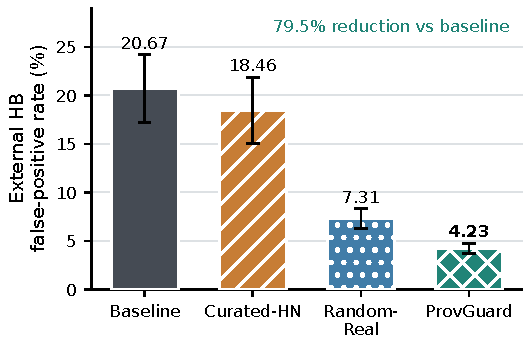
\includegraphics[width=\columnwidth]{figures/paper/external_hb.pdf}
\caption{External hard-benign FPR on \NExternal{} accessible prompts. Bars show five-seed means; error bars show sample SD, not confidence intervals. The equal-sized Random-Real control isolates the additional effect of confusion selection.}
\label{fig:external}
\end{figure}

\subsection{Targeted Selection versus Random-Real}
Random-Real itself reduces external FPR to \RandExtPct\%, demonstrating the value of realistic benign augmentation. ProvGuard lowers it further to \PGExtPct\%: \RandExtDropPP{} pp absolute and \RandExtDropRel\% relative. The crossed-bootstrap interval for this reduction, $\RandExtCI$, is positive. All five paired seed differences favor ProvGuard on this endpoint.

On aggregate HB, the point improvement is \RandHBDropPP{} pp, but the interval $\RandHBCI$ includes zero. Thus the external comparison supports a targeted-distribution advantage, while the predefined joint novelty verdict remains \emph{inconclusive}. Pointwise endpoint evidence must not be promoted to an adjusted, global superiority claim.

\begin{table}[t]
\caption{Aggregate crossed-bootstrap comparisons with ProvGuard. $\Delta$FPR = comparator minus ProvGuard; positive favors PG. Intervals are pointwise 95\%, over paired seeds and shared prompts, with \BootstrapN{} resamples. Rates are on the $0$--$1$ scale.}
\label{tab:stats}
\centering\footnotesize
\setlength{\tabcolsep}{1.7pt}
\renewcommand{\arraystretch}{1.13}
\begin{tabular}{@{}llrrl@{}}
\toprule
Comparator & Subset & $\Delta$FPR & 95\% CI & Interpretation \\
\midrule
Baseline & Overall & $+0.2775$ & $[0.2007,\,0.3512]$ & PG lower \\
Baseline & External & $+0.1644$ & $[0.1173,\,0.2144]$ & PG lower \\
Random-Real & Overall & $+0.0631$ & $[-0.0050,\,0.1408]$ & Inconclusive \\
Random-Real & External & $+0.0308$ & $[0.0096,\,0.0548]$ & PG lower \\
Curated-HN & Overall & $-0.0797$ & $[-0.1267,\,-0.0379]$ & Curated lower \\
Curated-HN & External & $+0.1423$ & $[0.0933,\,0.1933]$ & PG lower \\
\bottomrule
\end{tabular}

\end{table}

\subsection{Provenance-Sensitive Transfer}
Curated-HN has the lowest aggregate FPR, \CurHBPct\%, outperforming ProvGuard's \PGHBPct\%. This is a substantive result, not an exception to conceal. On the curated component alone, mean FPR is $\CurCuratedFPR$ for Curated-HN versus $\PGCuratedFPR$ for ProvGuard. Since \NCuratedHB{} of \NHB{} usable stress prompts are curated, the mixture rewards curated-style generalization.

The ordering reverses on external data: Curated-HN yields \CurExtPct\% FPR and ProvGuard \PGExtPct\%, a \CurExtDropPP{}-pp reduction (\CurExtDropRel\% relative). Both directional comparisons have intervals excluding zero. The contrast indicates provenance-sensitive augmentation effects. It does not establish that ranking alone explains the curated comparison, because the curated arm is smaller and differs in construction.

\subsection{Augmentation Size}
Figure~\ref{fig:diagnostics}(a) and Table~\ref{tab:ablation} show non-monotonic behavior: $K=250$ has the lowest aggregate HB FPR, \KSmallHBPct\%, whereas $K=500$ has the lowest external FPR, \KMediumExtPct\%. At $K=\PrimaryK$, these are \PGHBPct\% and \PGExtPct\%. These are descriptive test outcomes; the primary configuration remains $K=\PrimaryK$. Increasing augmentation size changes composition and does not guarantee a better operating point.

\subsection{OOD Behavior}
Structural-OOD benign FPR falls from \BaseStructPct\% to \PGStructPct\%, while domain-OOD F1 falls from $\BaseDom$ to $\PGDom$. The latter change is \BaseDomChangePP{} pp. Structural benign-side improvement therefore coexists with a domain-shift cost, and does not establish universal OOD robustness. The structural set contains attacks as well as benign transforms; an FPR gain alone does not characterize its complete security behavior.

\begin{table*}[t]
\caption{Nested augmentation-size ablation: five-seed mean $\pm$ sample SD. $K=\PrimaryK$ remains primary; no size is selected retrospectively from evaluation FPR. All rates are on the $0$--$1$ scale.}
\label{tab:ablation}
\centering\footnotesize
\setlength{\tabcolsep}{5pt}
\renewcommand{\arraystretch}{1.14}
\begin{tabular}{@{}rccccc@{}}
\toprule
$K$ & IID F1 & Attack recall & HB FPR & External FPR & Obf. recall \\
\midrule
250 & $0.9827\,\pm\,0.0021$ & $0.9854\,\pm\,0.0047$ & $0.1240\,\pm\,0.0407$ & $0.0538\,\pm\,0.0184$ & $0.9867\,\pm\,0.0051$ \\
500 & $0.9824\,\pm\,0.0005$ & $0.9869\,\pm\,0.0026$ & $0.1688\,\pm\,0.0592$ & $0.0346\,\pm\,0.0086$ & $0.9891\,\pm\,0.0028$ \\
1000 & $0.9826\,\pm\,0.0010$ & $0.9869\,\pm\,0.0016$ & $0.1384\,\pm\,0.0465$ & $0.0423\,\pm\,0.0053$ & $0.9877\,\pm\,0.0039$ \\
\bottomrule
\end{tabular}

\end{table*}

\begin{figure*}[t]
\centering
\begin{minipage}{.48\textwidth}\centering
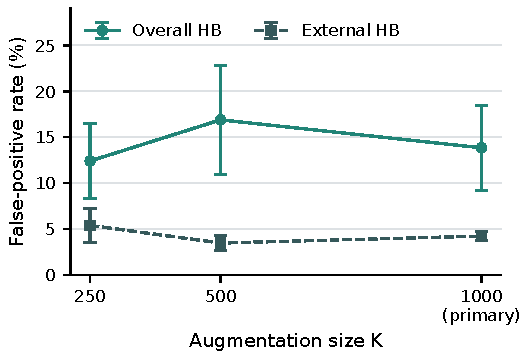
\includegraphics[width=\linewidth]{figures/paper/ablation.pdf}\\[-1pt]
\footnotesize (a) Augmentation-size sensitivity
\end{minipage}\hfill
\begin{minipage}{.48\textwidth}\centering
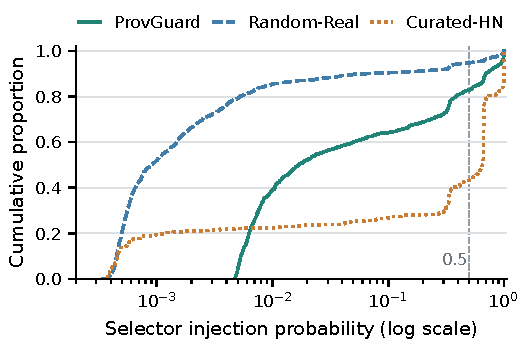
\includegraphics[width=\linewidth]{figures/paper/hardness_distribution.pdf}\\[-1pt]
\footnotesize (b) Selector-score distributions
\end{minipage}
\caption{(a) Performance varies non-monotonically with augmentation size; $K=\PrimaryK$ was predefined as primary. Error bars are five-seed sample SD. (b) Empirical CDFs of baseline ensemble scores; the log-scale axis exposes the skewed benign distributions. Curated-HN has \NCurAug{} rows; both real arms have \PrimaryK. The gray line marks $h=0.5$.}
\label{fig:diagnostics}
\end{figure*}

\subsection{Hardness and Error Analysis}
Selection changes the difficulty distribution (Fig.~\ref{fig:diagnostics}(b)). ProvGuard's mean selector score is \HardPGMean{}, versus \HardRandMean{} for Random-Real; medians are \HardPGMedian{} and \HardRandMedian{}. Only \HardPGFlagN{} of its \PrimaryK{} examples exceed mean probability $0.5$, versus \HardRandFlagN{} random examples. These are relatively confusing verified-benign examples, not uniformly misclassified inputs. This is a manipulation check, not independent evidence of generalization. Curated-HN is even harder by the same score (mean \HardCurMean) yet transfers worse externally, showing that score magnitude alone is insufficient.

Aligned aggregate HB predictions show an average of \FixedFP{} baseline false positives corrected and \NewFP{} new false positives introduced per seed. New errors are retained in the artifacts. Released curated taxonomies and ordered lexical proxies categorize remaining errors; these exploratory automated categories are distinct from validity labels and cannot establish a learned semantic mechanism.

\section{Discussion}
The controlled comparison separates two effects. Real benign data already reduces mismatch: Random-Real achieves much of the external gain. Confusion selection then adds an endpoint-specific improvement under equal augmentation size and matched corpus/length quotas. This is consistent with addressing underrepresented benign decision-boundary regions, but we do not measure intent representations or establish a causal shortcut-removal mechanism.

The aggregate/external reversal against Curated-HN is central. The mixture is curated-heavy, and curated augmentation resembles that component's construction. ProvGuard better covers external requests but leaves more curated false alarms. Reporting only the mixture would prefer Curated-HN and hide the targeted-domain benefit; reporting only external performance would hide the opposite cost. Both views are necessary.

Aggregate seed variation and heterogeneous provenance responses help explain why the matched random comparison remains uncertain even when its external interval is positive. Source/length matching controls selected marginals, not all language structure. The non-monotonic size ablation likewise favors treating composition as consequential rather than assuming more negatives always help.

Exploratory source-only augmentation checks ($K=250$; \SourceSeedN{} seeds per arm) further show asymmetric behavior. Dolly augmentation yields FPRs of $\SourceDollyDollyFPR$ on \NDollyExternal{} Dolly prompts and $\SourceDollyOasstFPR$ on \NOasstExternal{} OASST prompts; OASST augmentation yields $\SourceOasstDollyFPR$ and $\SourceOasstOasstFPR$, respectively. Only augmentation provenance is isolated: the original PIDS training split is retained, so this is not fully held-out-corpus training. These small, descriptive checks support inspecting provenance slices, not a general cross-corpus guarantee.

These results support a practical lesson: validate benign provenance slices alongside attack recall before choosing augmentation. They do not support replacing trust-boundary controls with a classifier or treating stress FPR as a production rate. Generalization to new corpora, production traffic, and stronger architectures remains unestablished.

\section{Limitations}
The external subset contains only \NExternal{} prompts; \NWithheld{} LMSYS texts cannot be evaluated. Dolly and OASST1 are shared candidate/evaluation corpora, not a representative sample of production traffic. Lexical exclusion cannot ensure semantic independence. Automated adjudicators can share errors, are not human annotators, and lack an exposed exact model identifier. A \HardPGFlagN{}-row high-score queue is provided for a future human audit; no completed human labels are claimed.

The primary architecture is DistilBERT: an optional DeBERTa attempt failed technically and supplies no transfer evidence. Five seeds limit uncertainty resolution; the selector ensemble and one random augmentation draw are fixed across those seeds. Additional random-sample checks lack completed reviews. Curated-HN uses \NCurAug{} examples and is not size matched. The joint Random-Real comparison is inconclusive, domain-OOD F1 decreases, and source/length matching does not guarantee syntactic matching. No adaptive-attacker, unseen-transform, or end-to-end security claim is made.

\section{Conclusion}
ProvGuard shows that the provenance and selection of benign augmentation materially shape prompt-injection over-defense. Confusion-selected real hard negatives lower external HB FPR from \BaseExtPct\% to \PGExtPct\% while retaining measured IID attack recall. They improve over matched Random-Real on the targeted external subset, but the aggregate comparison remains inconclusive and curated augmentation wins the curated-heavy mixture. Non-monotonic size effects and a domain-OOD cost further qualify the result. The contribution is a reproducible data-selection study with distribution-specific benefits, rather than a universally stronger detector.

\IEEEtriggeratref{3}
\bibliographystyle{IEEEtran}
\bibliography{ProvGuard}
\end{document}
